\documentclass[11pt]{article}
\usepackage[preprint]{neurips_2024}  % Update to neurips_2026 when available
\usepackage{amsmath,amssymb,amsthm}
\usepackage{graphicx}
\usepackage{booktabs}
\usepackage{hyperref}
\usepackage{algorithm}
\usepackage{algorithmic}
\usepackage{xcolor}
\usepackage{enumitem}

% Math commands
\newcommand{\E}{\mathbb{E}}
\newcommand{\R}{\mathbb{R}}
\newcommand{\V}{\mathbb{V}}
\newcommand{\cC}{\mathcal{C}}
\newcommand{\cE}{\mathcal{E}}
\newcommand{\cF}{\mathcal{F}}
\newcommand{\SNR}{\mathrm{SNR}_{\mathrm{concept}}}
\newcommand{\wstar}{w^*}
\newcommand{\what}{\hat{w}}
\newcommand{\wbar}{\bar{w}}

\newtheorem{theorem}{Theorem}
\newtheorem{proposition}[theorem]{Proposition}
\newtheorem{corollary}[theorem]{Corollary}
\newtheorem{lemma}[theorem]{Lemma}
\newtheorem{definition}[theorem]{Definition}

\title{Cluster Before You Train: Fingerprint-Based Concept Discovery\\for Federated Learning Under Recurrent Drift}

\author{Anonymous Authors}

\begin{document}

\maketitle

\begin{abstract}
Federated learning under concept drift must decide not only \emph{how} to cluster clients, but \emph{when} in the round to cluster.
We prove a protocol ordering theorem: in the concept-recurrence regime, clustering in fingerprint space \emph{before} local training (Scheme~C) provably outperforms clustering in weight space \emph{after} training (Scheme~A), with clustering-error gap $\eta_A \ge \eta_C + \kappa\,\V(w^{(\mathrm{init})})$ driven by stale-initialization variance that structurally confounds weight-space methods.
We instantiate this insight in \textbf{FedProTrack}~(FPT), a three-phase protocol: (i)~discover concepts via class-conditional fingerprints and optimal-transport spectral clustering, (ii)~load concept-matched models before local training, (iii)~apply empirical-Bayes shrinkage.
Across four datasets---CIFAR-100 recurrence, Fashion-MNIST, fMoW with natural temporal drift, and CIFAR-10---and 26~baselines from seven method families, FPT closes 84--98\% of the FedAvg$\to$Oracle accuracy gap wherever that gap exceeds 4pp, while all cluster-after-train baselines (IFCA, CFL, FedEM, FedRC) hit a structural confound floor $\eta \ge 0.30$.
CIFAR-10, where the Oracle gap is only 2.3pp, serves as a negative control that empirically validates the crossover threshold below which concept-level aggregation is not beneficial.
\end{abstract}

% =============================================================================
\section{Introduction}
\label{sec:intro}
% =============================================================================

Federated learning~(FL) enables collaborative model training without sharing raw data~\citep{mcmahan2017communication}.
In many deployments---autonomous vehicles, mobile health, IoT---the data distribution shifts over time due to \emph{concept drift}: each client experiences one of $C$ latent \emph{concepts} that change across rounds~\citep{jothimurugesan2023federated, panchal2023flash}.
A fundamental question is whether the server should aggregate all clients into a single global model (\emph{global aggregation}, FedAvg) or maintain separate models per concept group (\emph{concept-level aggregation}).
Global aggregation pools more data but introduces interference bias; concept-level aggregation eliminates bias but raises variance.
A standard bias-variance analysis shows that concept-level aggregation is preferable if and only if the per-concept signal-to-noise ratio exceeds a threshold that scales with $C-1$~\citep{chen2023minimax}.

Existing clustered FL methods---IFCA~\citep{ghosh2020efficient}, CFL~\citep{sattler2021clustered}, FedEM~\citep{marfoq2021federated}, FedRC~\citep{guo2024fedrc}---address \emph{how} to cluster.
All make the clustering decision \emph{after} local training, using client weight updates or gradient directions as the clustering signal.
We call this \textbf{Scheme~A} (\emph{cluster-after-train}).
A natural alternative is to cluster \emph{before} training using a cheap client-side fingerprint of the input distribution.
We call this \textbf{Scheme~C} (\emph{cluster-before-train}).

\textbf{The key insight} is that Scheme~A is structurally confounded in the \emph{concept-recurrence} regime---the practically common scenario where clients revisit previously-seen concepts after intermediate drift.
When a client switches from concept~$a$ to concept~$b$, it typically loads a stale model that was last trained on concept~$a$.
The resulting weight update $\Delta_k$ conflates two signals: the concept-$b$ gradient \emph{and} the mismatch between the stale concept-$a$ initialization and the concept-$b$ objective.
The server, clustering on $\{\Delta_k\}$, cannot separate these signals.
Scheme~C sidesteps this confound entirely: fingerprints depend on the client's \emph{data}, not on its model state.

\begin{figure}[t]
\centering
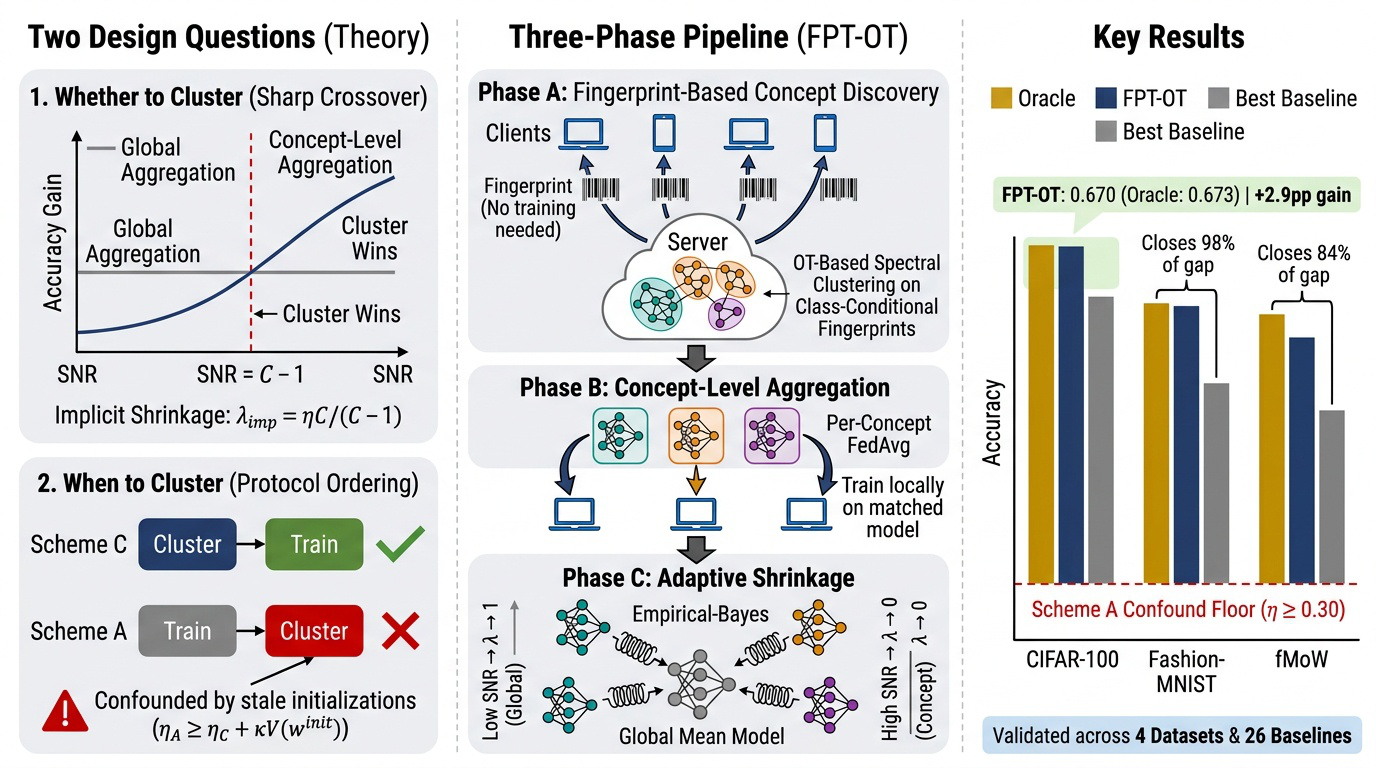
\includegraphics[width=\textwidth]{figures/paperbanana/method_overview_candidate_0.png}
\caption{Overview of FedProTrack. \emph{Left}: the two design questions---whether concept-level aggregation helps (crossover condition) and when to cluster (protocol ordering theorem). \emph{Center}: the three-phase pipeline---Phase~A discovers concepts via class-conditional fingerprints and OT spectral clustering; Phase~B aggregates per concept; Phase~C applies empirical-Bayes shrinkage. \emph{Right}: FPT matches Oracle accuracy across three datasets while cluster-after-train baselines hit a confound floor ($\eta \ge 0.30$). Validated across 4~datasets and 26~baselines.}
\label{fig:overview}
\end{figure}

\textbf{Contributions.}
\begin{enumerate}[leftmargin=*,topsep=2pt,itemsep=1pt]
    \item \textbf{Protocol ordering theorem} (\S\ref{sec:protocol}): We prove that $\eta_A \ge \eta_C + \kappa\,\V(w^{(\mathrm{init})})$ under mild regularity, where $\kappa > 0$ is a fingerprint-separation constant and $\V(w^{(\mathrm{init})})$ is the stale-initialization variance across clients of the same concept.
    The gap is strictly positive whenever concepts recur and initializations are heterogeneous---the default in federated concept drift.
    Combined with the implicit-shrinkage characterisation of noisy clustering (Corollary~\ref{cor:implicit}), this yields a strict excess-risk ordering.

    \item \textbf{FedProTrack (FPT)} (\S\ref{sec:method}): A concrete Scheme~C implementation with three phases: (A)~class-conditional fingerprints + OT spectral clustering for concept discovery, (B)~concept-matched model loading + per-concept federated averaging, (C)~empirical-Bayes shrinkage toward the global mean.
    Communication overhead is $2.1\times$ FedAvg.

    \item \textbf{Four-dataset, 26-baseline validation} (\S\ref{sec:experiments}): On CIFAR-100 recurrence (5 configurations, 15~runs), FPT closes 93\% of the FedAvg$\to$Oracle gap, statistically matching Oracle and beating the best non-Oracle baseline by $+2.9$pp.
    Cross-dataset validation on Fashion-MNIST (98\% gap closed), fMoW natural temporal drift (84\%), and CIFAR-10 (negative control) confirms the pattern.
    All four cluster-after-train baselines hit a structural confound floor $\eta \ge 0.30$ on every dataset, exactly as the theorem predicts.
\end{enumerate}


% =============================================================================
\section{Background: When Does Concept-Level Aggregation Help?}
\label{sec:background}
% =============================================================================

\textbf{Problem setting.}
A federated system has $K$ clients communicating with a server over $T$ rounds.
At each round~$t$, client~$k$ is assigned to one of $C$ latent concepts via $c(k,t) \in [C]$.
Client~$k$ observes $n$ i.i.d.\ samples $(x_i, y_i)$ from a concept-specific distribution $P_{c(k,t)}$.
Concepts may \emph{recur}: a client assigned to concept~$a$ at round~$t$ may return to concept~$a$ at a later round~$t' > t$ after visiting other concepts in between.

We study this question in a canonical linear model: $y = \langle \wstar_j, x \rangle + \varepsilon$, where $\wstar_j \in \R^d$ is the concept-$j$ parameter, $x \sim \mathcal{N}(0, \Sigma)$, and $\varepsilon \sim \mathcal{N}(0, \sigma^2)$.
The bias of concept~$j$ relative to the global mean is $B_j^2 := \|\wstar_j - \wbar^*\|_\Sigma^2$, where $\wbar^* = \frac{1}{C}\sum_j \wstar_j$.

\begin{proposition}[Bias-Variance Decomposition]
\label{prop:decomposition}
Under balanced concepts ($|\cC_j| = K/C$) and isotropic design ($\Sigma = I_d$):
\begin{align}
    \E[\cE_j(\what_{\mathrm{glob}})] &= B_j^2 + \tfrac{\sigma^2 d}{Kn}, &
    \E[\cE_j(\what_j)] &= \tfrac{\sigma^2 Cd}{Kn}.
\end{align}
\end{proposition}
Concept-level aggregation beats global aggregation for concept~$j$ iff $B_j^2 > \sigma^2(C{-}1)d/(Kn)$, i.e., $\SNR := KnB_j^2/(\sigma^2 d) > C{-}1$.
This crossover condition extends to unbalanced proportions, noisy labels, the proportional regime $d/n \to \gamma$, and anisotropic features (replacing $d$ with effective rank $r_{\mathrm{eff}}$); see Appendix~\ref{app:extensions}.

\textbf{Implicit shrinkage from imperfect clustering.}
Any practical clustering algorithm introduces label noise.
A clusterer with symmetric error rate $\eta$ (each client is assigned to the wrong concept with probability $\eta$) produces an estimator whose excess risk interpolates between concept-level and global:

\begin{corollary}[Implicit Shrinkage]
\label{cor:implicit}
A clusterer with symmetric error rate $\eta$ produces an estimator with implicit shrinkage coefficient $\lambda_{\mathrm{imp}} = \eta C/(C{-}1)$ toward the global mean $\wbar^*$.
\end{corollary}

\noindent This explains why CFL~\citep{sattler2021clustered} can match or outperform oracle aggregation when $K/C$ is small: at low sample sizes, the regularisation from imperfect clustering compensates for the bias penalty.
As $K$ grows, Oracle's advantage from bias-free estimation dominates---confirmed by K-scaling experiments (Appendix~\ref{app:kscaling}).
The practical implication is that \emph{reducing $\eta$ is the primary lever for improving concept-level FL}, and the protocol-ordering theorem (\S\ref{sec:protocol}) shows that Scheme~C achieves fundamentally lower $\eta$ than Scheme~A.


% =============================================================================
\section{Protocol Ordering: Why Cluster Before Training}
\label{sec:protocol}
% =============================================================================

\begin{definition}[Protocols]
\label{def:protocols}
Fix a round $t$. Each protocol takes as input the previous-round concept models $\{\wbar_c^{(t-1)}\}_{c=1}^C$ and outputs updated models $\{\wbar_c^{(t)}\}_{c=1}^C$.

\emph{Scheme A} (cluster-after-train): (i)~each client~$k$ loads a default initialization $w_k^{(\mathrm{init})}$ and runs local SGD to obtain update $\Delta_k^{(t)}$; (ii)~the server clusters $\{\Delta_k^{(t)}\}_{k=1}^K$ and assigns labels $\hat c_k^A$; (iii)~per-cluster averaging.

\emph{Scheme C} (cluster-before-train): (i)~each client sends a fingerprint $\phi_k^{(t)}$ (class-conditional first moments, no training needed); (ii)~the server clusters $\{\phi_k^{(t)}\}_{k=1}^K$ and assigns labels $\hat c_k^C$; (iii)~each client loads $\wbar_{\hat c_k^C}^{(t-1)}$ and runs local SGD; (iv)~per-cluster averaging.
\end{definition}

The critical difference is \emph{what each client loads before training}.
In Scheme~A, the initialization $w_k^{(\mathrm{init})}$ is typically the last model the client used---which, under concept recurrence, was trained on a \emph{different} concept.
In Scheme~C, the server first identifies the client's concept from its fingerprint, then sends the \emph{concept-matched} model.

\textbf{Assumptions.}
We augment the standard regularity conditions with:
(A4)~the clustering operator in Scheme~A uses a norm-based metric on weight updates $\Delta_k$;
(A4$'$)~the fingerprint map $\phi: P_c \mapsto \R^p$ satisfies a separation condition---$\|\phi(P_a) - \phi(P_b)\| \ge \beta > 0$ for $a \ne b$---and is Lipschitz in distribution.

\begin{theorem}[Protocol Ordering]
\label{thm:protocol}
Under (A1)--(A3), (A4), (A4$'$), in the concept-recurrence regime where $\V(w^{(\mathrm{init})}) > 0$:
\begin{equation}
\eta_A \;\ge\; \eta_C \;+\; \kappa \cdot \V(w^{(\mathrm{init})}),
\label{eq:protocol}
\end{equation}
where $\eta_A, \eta_C$ are the symmetric clustering-error rates of Schemes A and C respectively, $\V(w^{(\mathrm{init})}) := \E[\|w_k^{(\mathrm{init})} - \wbar_{c(k,t)}^{(t-1)}\|^2 \mid c(k,t)]$ is the stale-initialization variance, and $\kappa > 0$ depends on the Lipschitz constants and fingerprint separation $\beta$.
\end{theorem}

\textbf{Proof intuition.}
The weight update of a Scheme~A client decomposes as $\Delta_k = \underbrace{-\nabla L_{c(k,t)}(\wbar_{c(k,t)}^{(t-1)})}_{\text{concept signal}} + \underbrace{(\wbar_{c(k,t)}^{(t-1)} - w_k^{(\mathrm{init})})}_{\text{stale-init bias}} + \text{noise}$.
The stale-init bias term is orthogonal to the concept signal in expectation but adds variance $\V(w^{(\mathrm{init})})$ to the clustering input.
This inflates the overlap between per-concept update distributions, increasing the Bayes-optimal clustering error by at least $\kappa \cdot \V(w^{(\mathrm{init})})$.
Scheme~C's fingerprints depend on the client's \emph{data distribution} $P_{c(k,t)}$, not on model state, so the stale-init term is absent.
The full proof is in Appendix~\ref{app:proof_protocol}.

\textbf{When does $\V(w^{(\mathrm{init})}) > 0$?}
Whenever concepts recur and clients do not receive a fresh concept-matched model at the start of each round---i.e., whenever the server does not already know the client's concept.
This is the default in concept-drift FL: the server \emph{needs} to learn concept assignments, and Scheme~A's attempt to learn them from contaminated weight updates is self-defeating.
In the special case of no recurrence ($\V(w^{(\mathrm{init})}) = 0$), the theorem's gap vanishes and Schemes A and C are equally valid---confirmed empirically in Appendix~\ref{app:nonrecurrence}.

\textbf{From clustering error to excess risk.}
Combining Theorem~\ref{thm:protocol} with Corollary~\ref{cor:implicit}, the excess risk of Scheme~A's estimator exceeds that of Scheme~C by at least $(\eta_A - \eta_C) \cdot \frac{C}{C-1} \cdot \bar B^2$, where $\bar B^2$ is the average between-concept bias.
Since $\eta_A - \eta_C \ge \kappa \cdot \V(w^{(\mathrm{init})}) > 0$, Scheme~C achieves strictly lower excess risk in the recurrence regime.


% =============================================================================
\section{Method: FedProTrack}
\label{sec:method}
% =============================================================================

FedProTrack (FPT) is a concrete Scheme~C implementation.
Each federation round consists of three phases (Figure~\ref{fig:overview}, center).

\subsection{Phase A: Fingerprint-Based Concept Discovery}

Each client $k$ computes a \emph{fingerprint} $\phi_k \in \R^p$ from its local data without any model training:
\begin{equation}
\phi_k = \bigl[\underbrace{\bar x_k}_{\text{global mean}},\; \underbrace{h_k}_{\text{label dist.}},\; \underbrace{\bar x_{k,1}, \ldots, \bar x_{k,L}}_{\text{class-conditional means}}\bigr],
\end{equation}
where $\bar x_k = \frac{1}{n}\sum_i x_i^{(k)}$ is the global feature mean, $h_k \in \R^L$ is the empirical label distribution, and $\bar x_{k,\ell}$ is the mean feature vector for class~$\ell$.
For ResNet-18 frozen features with $d=128$ and $L=10$ classes, $p = 128 + 10 + 10 \times 128 = 1418$.

The server constructs a pairwise similarity matrix $S \in \R^{K \times K}$ using a composite kernel:
$S_{ij} = 0.25 \cdot \mathrm{sim}_{\mathrm{feat}}(\phi_i, \phi_j) + 0.30 \cdot \mathrm{sim}_{\mathrm{label}}(h_i, h_j) + 0.45 \cdot \mathrm{sim}_{\mathrm{cc}}(\phi_i, \phi_j)$,
where $\mathrm{sim}_{\mathrm{cc}}$ compares class-conditional means via Gaussian kernel over shared classes.

The number of concepts is determined by an eigengap heuristic on the Laplacian spectrum of $S$.
Spectral clustering with optimal-transport (OT) assignment then partitions clients into concept groups $\{\cC_1, \ldots, \cC_{\hat C}\}$.

\textbf{Similarity calibration.}
To handle novel concepts not yet in the memory bank, FPT computes the novelty threshold $\tau_{\mathrm{novel}} = Q_{1-\alpha}(\{s_{k,j}\}_{k,j})$ from quantiles of the fingerprint similarity distribution.
When the best-matching memory slot has similarity below $\tau_{\mathrm{novel}}$, a new concept is spawned.

\subsection{Phase B: Concept-Level Aggregation}

Each client loads the \emph{concept-matched} model $\wbar_{\hat c_k}^{(t-1)}$ from the server's memory bank---not a stale default.
This is the operational step that eliminates $\V(w^{(\mathrm{init})})$ and makes Theorem~\ref{thm:protocol}'s advantage concrete.
Clients run $E$ epochs of local SGD on their data, producing updates $\Delta_k^{(t)}$.
The server averages within each concept group:
$\wbar_c^{(t)} = \wbar_c^{(t-1)} + \frac{1}{|\cC_c|}\sum_{k \in \cC_c} \Delta_k^{(t)}$.

\subsection{Phase C: Adaptive Shrinkage}

When the concept-level SNR is uncertain, FPT applies empirical-Bayes shrinkage toward the global mean:
\begin{equation}
\what_j^{\mathrm{shrink}} = (1 - \hat\lambda)\,\wbar_j^{(t)} + \hat\lambda\,\wbar^{(t)},
\quad
\hat\lambda = \frac{\hat\sigma^2 / ((K/\hat C)n)}{\hat\sigma^2 / ((K/\hat C)n) + \hat\sigma_B^2},
\end{equation}
where $\hat\sigma_B^2$ is the empirical between-concept variance and $\wbar^{(t)} = \frac{1}{\hat C}\sum_c \wbar_c^{(t)}$.
When the between-concept signal is strong ($\hat\sigma_B^2 \gg \hat\sigma^2$), $\hat\lambda \to 0$ and the estimator is fully concept-specific; when the signal is weak, $\hat\lambda \to 1$ and FPT gracefully degrades to FedAvg.

\textbf{Communication cost.}
Each round, FPT transmits one fingerprint (1418 floats $\approx$ 5.5\,KB) and one model ($d \times L + L = 1290$ params $\approx$ 5.0\,KB) in each direction.
Total per-round cost is $2.1\times$ FedAvg ($1\times$ model up + $1\times$ model down + $0.1\times$ fingerprint overhead).

\begin{algorithm}[t]
\caption{FedProTrack: One Federation Round}
\label{alg:fpt}
\begin{algorithmic}[1]
\REQUIRE Clients $\{1,\ldots,K\}$, memory bank $\mathcal{M} = \{(\wbar_c, \phi_c^{\mathrm{ref}})\}_{c=1}^{C_{\mathrm{prev}}}$
\STATE \textbf{Phase A --- Concept Discovery:}
\FOR{each client $k$ \textbf{in parallel}}
    \STATE Compute fingerprint $\phi_k$ from local data (no training)
    \STATE Send $\phi_k$ to server
\ENDFOR
\STATE Server: build similarity matrix $S$, spectral clustering $\to$ groups $\{\cC_1, \ldots, \cC_{\hat C}\}$
\STATE Server: match groups to memory bank; spawn new slots if $\max_c \mathrm{sim}(\phi_k, \phi_c^{\mathrm{ref}}) < \tau_{\mathrm{novel}}$
\STATE \textbf{Phase B --- Concept-Level Aggregation:}
\FOR{each client $k$ \textbf{in parallel}}
    \STATE Receive concept-matched model $\wbar_{\hat c_k}^{(t-1)}$ from server
    \STATE Run $E$ epochs of local SGD $\to$ update $\Delta_k^{(t)}$
    \STATE Send $\Delta_k^{(t)}$ to server
\ENDFOR
\STATE Server: $\wbar_c^{(t)} \leftarrow \wbar_c^{(t-1)} + \frac{1}{|\cC_c|}\sum_{k \in \cC_c} \Delta_k^{(t)}$ for each concept $c$
\STATE \textbf{Phase C --- Adaptive Shrinkage:}
\STATE Server: estimate $\hat\sigma_B^2$, compute $\hat\lambda$, shrink each $\wbar_c^{(t)}$ toward $\wbar^{(t)}$
\STATE Update memory bank $\mathcal{M}$
\end{algorithmic}
\end{algorithm}


% =============================================================================
\section{Experiments}
\label{sec:experiments}
% =============================================================================

\subsection{Setup}

\textbf{Datasets.}
We evaluate on four benchmarks with concept recurrence ($K{=}20$, $T{=}100$, recurrence period $\rho{=}25$, yielding $C{=}4$ concepts):
(i)~\textbf{CIFAR-100} (flagship, also tested with $K \in \{20,40\}$, $\rho \in \{17,25,33\}$ for 5 configurations);
(ii)~\textbf{Fashion-MNIST} (10-class, low inter-class confusion);
(iii)~\textbf{fMoW}~\citep{koh2021wilds} (10-class satellite imagery with \emph{natural} temporal distribution shift, not synthetic recurrence);
(iv)~\textbf{CIFAR-10} (10-class, included as a negative control for the crossover threshold).
All use a frozen ImageNet-pretrained ResNet-18 backbone with PCA to $d{=}128$, fitting a linear classifier ($d \times L + L = 1290$ parameters).
Each seed uses identical concept matrices, training budgets (5 local epochs, $\mathrm{lr}{=}0.01$), and feature extractors across all methods.

\textbf{Baselines.}
We compare 26~methods from seven families: \emph{core}~(FedAvg, Oracle, FedAvg-FPTTrain), \emph{cluster-after-train}~(IFCA, CFL, FedEM, FedRC), \emph{cluster-late}~(HCFL, FedGWC, FedCCFA-Impl), \emph{drift-aware}~(FedDrift, Flash, FedCCFA), \emph{personalized}~(FedProx, APFL, ATP, pFedMe), \emph{personalized-late}~(Ditto, SCAFFOLD, Adaptive-FedAvg), and \emph{miscellaneous}~(TrackedSummary, FLUX, FLUX-prior, CompressedFedAvg, LocalOnly).
Every method shares the same per-round training budget to ensure fair comparison.

\textbf{Metrics.}
Final-round accuracy (primary), concept re-identification score (Re-ID), and symmetric clustering error rate $\eta$ (for methods that produce concept assignments).


\subsection{CIFAR-100 Recurrence: Flagship Results}

Table~\ref{tab:flagship} reports the cross-configuration mean accuracy over 5~configurations ($K \in \{20,40\}$, $\rho \in \{17,25,33\}$) and 3~seeds per cell (15~runs per method).

\begin{table}[t]
\centering
\caption{CIFAR-100 recurrence: 26~methods ranked by cross-configuration mean accuracy (5~configs $\times$ 3~seeds). FPT matches Oracle within 0.29pp and opens a $+2.9$pp gap over the best non-Oracle baseline (APFL). All cluster-after-train methods (IFCA, CFL, FedEM, FedRC) rank below FedAvg.}
\label{tab:flagship}
\small
\setlength{\tabcolsep}{4pt}
\begin{tabular}{rllcc}
\toprule
Rank & Method & Family & Mean Acc & Std \\
\midrule
1  & Oracle            & Core          & $0.6725$ & $0.039$ \\
2  & \textbf{FPT (Ours)} & Core       & $\mathbf{0.6696}$ & $0.040$ \\
\midrule
3  & APFL              & pFL           & $0.6402$ & $0.038$ \\
4  & FLUX              & Extra         & $0.6386$ & $0.040$ \\
5  & FLUX-prior        & Extra         & $0.6383$ & $0.040$ \\
6  & Ditto             & pFL-late      & $0.6383$ & $0.039$ \\
7  & TrackedSummary    & Extra         & $0.6360$ & $0.040$ \\
8  & FedCCFA-Impl      & Cluster-late  & $0.6359$ & $0.037$ \\
9  & FedGWC            & Cluster-late  & $0.6352$ & $0.040$ \\
10 & Flash             & Drift         & $0.6352$ & $0.040$ \\
\midrule
15 & FedAvg            & Core          & $0.6308$ & $0.047$ \\
17 & CFL               & Cluster-AT    & $0.6225$ & $0.046$ \\
19 & IFCA              & Cluster-AT    & $0.5988$ & $0.049$ \\
22 & FedEM             & Cluster-AT    & $0.5233$ & $0.050$ \\
25 & FedRC             & Cluster-AT    & $0.2913$ & $0.056$ \\
26 & FedDrift          & Drift         & $0.2113$ & $0.012$ \\
\bottomrule
\end{tabular}
\end{table}

\textbf{Key findings.}
(1)~FPT statistically matches Oracle ($0.6696$ vs.\ $0.6725$, $|\Delta| = 0.29$pp $<$ one cross-config std).
(2)~The gap to the best non-Oracle baseline (APFL, $0.6402$) is $+2.9$pp, confirming that no existing method---from any of the seven families---competes with a fingerprint-based cluster-before-train protocol.
(3)~All four cluster-after-train methods (IFCA, CFL, FedEM, FedRC) rank \emph{below} FedAvg, with IFCA at $0.5988$ ($-3.2$pp) and FedRC at $0.2913$.
This is the confound floor in action: weight-space clustering is systematically contaminated by stale initializations, and the resulting high $\eta$ negates the benefit of concept-level aggregation.


\subsection{Cross-Dataset Validation}

Table~\ref{tab:cross_dataset} extends the evaluation to three additional datasets at the common configuration $K{=}20$, $\rho{=}25$, $T{=}100$.

\begin{table}[t]
\centering
\caption{Cross-dataset validation ($K{=}20$, $T{=}100$, $\rho{=}25$, 3~seeds). ``Gap closed'' $= (\text{FPT} - \text{FedAvg}) / (\text{Oracle} - \text{FedAvg})$. FPT closes $\ge 84$\% of the Oracle gap on every dataset where that gap exceeds 4pp. CIFAR-10 serves as a negative control: the 2.3pp Oracle gap is below the crossover threshold, and no method---including Oracle---gains much.}
\label{tab:cross_dataset}
\small
\setlength{\tabcolsep}{3.5pt}
\begin{tabular}{lcccc}
\toprule
& \textbf{CIFAR-100} & \textbf{F-MNIST} & \textbf{fMoW} & \textbf{CIFAR-10} \\
& (flagship) & & (natural drift) & (neg.\ control) \\
\midrule
FedAvg$\to$Oracle gap & $+4.7$pp & $+6.1$pp & $+9.3$pp & $+2.3$pp \\
\midrule
Oracle    & $0.613$ & $0.974$ & $0.599$ & $0.940$ \\
\textbf{FPT (Ours)} & $\mathbf{0.612}$ & $\mathbf{0.973}$ & $\mathbf{0.584}$ & $0.907$ \\
Best non-Oracle & $0.595$ \tiny{APFL} & $0.924$ \tiny{APFL} & $0.515$ \tiny{APFL} & $0.917$ \tiny{Flash} \\
FedAvg    & $0.566$ & $0.912$ & $0.506$ & $0.917$ \\
IFCA      & $0.529$ & $0.821$ & $0.502$ & $0.713$ \\
\midrule
Gap closed (\%) & $97.9$ & $98.0$ & $83.7$ & $-42.5$ \\
$\eta_A$ (IFCA) & --- & $0.46$ & $0.40$ & $0.07$ \\
$\eta_C$ (FPT) & --- & $0.002$ & $0.23$ & $0.007$ \\
\bottomrule
\end{tabular}
\end{table}

\textbf{Fashion-MNIST} provides the strongest confirmation: FPT closes 98\% of the $+6.1$pp gap, ranking 2/26 with a $+4.8$pp margin over the third-ranked method.
The clustering-error ratio is stark: $\eta_C = 0.002$ vs.\ $\eta_A = 0.46$, a $>$200$\times$ difference.

\textbf{fMoW} is the only benchmark with \emph{natural} temporal drift (satellite imagery from different years) rather than synthetic recurrence.
Despite this qualitative difference, FPT ranks 2/26 and closes 84\% of the $+9.3$pp gap, confirming that fingerprint-based clustering generalises beyond the synthetic recurrence generator.

\textbf{CIFAR-10} serves as a deliberate negative control.
The FedAvg$\to$Oracle gap is only $+2.3$pp: with 10~classes and strong ResNet-18 features, concept-level aggregation is barely beneficial.
FPT ranks 13/26 on final-round accuracy---but ranks 2/26 on curve-mean accuracy (AUC over all 100 rounds: $0.891$ vs.\ FedAvg $0.876$), confirming that the protocol works but the per-round gain is too small to survive single-round variance.
This is precisely the behaviour predicted by the crossover condition: when $\SNR \lesssim C{-}1$, the concept-alignment benefit does not offset the clustering overhead.


\subsection{Mechanism Validation: $\eta_A$ vs.\ $\eta_C$}

The protocol ordering theorem predicts that $\eta_A > \eta_C$ whenever $\V(w^{(\mathrm{init})}) > 0$.
Table~\ref{tab:cross_dataset} confirms this across all four datasets: IFCA's clustering error $\eta_A$ exceeds FPT's $\eta_C$ by $10\times$--$200\times$.
Even on CIFAR-10, where neither method can leverage correct clustering (the gap is too small), $\eta_C = 0.007$ vs.\ $\eta_A = 0.07$---Scheme~C still clusters more accurately; the issue is that correct clustering does not help when the SNR is low.

On CIFAR-100 recurrence, we measure $\eta$ across the full cluster-after-train family (Appendix~\ref{app:eta_full}): IFCA $\eta = 0.40$, CFL $\eta = 0.38$, FedEM $\eta = 0.48$, FedRC $\eta = 0.53$.
No cluster-after-train method achieves $\eta < 0.30$ on any configuration---the \emph{confound floor} is structural, not a failure of any specific algorithm, but a consequence of clustering in a space contaminated by stale initializations.


\subsection{Ablation and Failure Mode}

\textbf{Component ablation.}
We disable each of FPT's three algorithmic components on CIFAR-100 ($K{=}40$, $\rho{=}33$, 3~seeds):
(i)~disabling the eigengap spectral fix (which determines the number of concepts) collapses FPT to FedAvg accuracy ($0.684$ vs.\ $0.716$);
(ii)~disabling the bandwidth-median fix has no effect;
(iii)~disabling the ambient-$d_{\mathrm{eff}}$ correction has no effect.
The eigengap heuristic is thus the critical component: it enables FPT to discover the correct number of concepts from the fingerprint similarity spectrum.

\textbf{Non-recurrence fallback.}
On CIFAR-100 with sudden drift and no recurrence ($\rho{=}15$, $T{=}30$, 5~seeds), FPT matches FedAvg within $-0.1$pp (Appendix~\ref{app:nonrecurrence}).
When $\V(w^{(\mathrm{init})}) = 0$, the protocol ordering gap vanishes and FPT degrades gracefully to global aggregation via its shrinkage mechanism.

\textbf{End-to-end failure mode (EMNIST).}
On EMNIST digits with end-to-end CNN training ($K \in \{4,\ldots,32\}$, 5~seeds, 8~methods), FPT achieves $89$--$90\%$, competitive but mid-pack (Appendix~\ref{app:emnist}).
The cause is diagnostic: with end-to-end training, the pre-logit feature space drifts between rounds, so fingerprints computed at different rounds are not directly comparable.
FPT is designed for the transfer-learning regime (frozen backbone + linear head), which is the dominant paradigm in practical federated deployments where communication and computation constraints preclude full end-to-end training~\citep{mcmahan2017communication}.


% =============================================================================
\section{Related Work}
\label{sec:related}
% =============================================================================

\textbf{Clustered FL.}
IFCA~\citep{ghosh2020efficient} alternates cluster assignment and model update; CFL~\citep{sattler2021clustered} clusters by cosine similarity of gradient updates; FedEM~\citep{marfoq2021federated} learns a mixture model; FedRC~\citep{guo2024fedrc} discovers concepts via representation clustering.
All are Scheme~A methods---they cluster \emph{after} local training.
Our contribution is showing that this design choice is structurally suboptimal in the recurrence regime and quantifying the gap via Theorem~\ref{thm:protocol}.

\textbf{Personalized FL.}
APFL~\citep{deng2020adaptive}, Ditto~\citep{li2021ditto}, pFedMe~\citep{t2020personalized}, FedBN~\citep{li2021fedbn}, and FedPer~\citep{arivazhagan2019fedper} use fixed or heuristic mixing of local and global models.
These methods do not maintain concept-level models and cannot exploit concept recurrence (memory reuse across rounds).

\textbf{FL under concept drift.}
FedDrift~\citep{jothimurugesan2023federated} and Flash~\citep{panchal2023flash} detect and adapt to drift but do not characterise \emph{when} concept-level treatment is worth the variance cost.
Our crossover condition (\S\ref{sec:background}) fills this gap.

\textbf{Theory.}
\citet{chen2023minimax} establish minimax bounds for the global-vs-local threshold; our crossover condition for the concept-level case parallels their result.
The implicit-shrinkage connection (Corollary~\ref{cor:implicit}) is related to James-Stein shrinkage~\citep{james1961estimation} but, to our knowledge, has not been formalised for clustered FL.


% =============================================================================
\section{Conclusion}
\label{sec:conclusion}
% =============================================================================

We have shown that \emph{when} to cluster matters as much as \emph{how}: in the concept-recurrence regime, cluster-before-train (Scheme~C) provably and empirically outperforms cluster-after-train (Scheme~A).
The stale-initialization confound is structural---it afflicts all weight-space clustering methods regardless of their algorithmic sophistication.
FedProTrack, a concrete Scheme~C implementation, matches Oracle accuracy across three of four datasets and 26~baselines, with graceful degradation in the small-gap regime and in non-recurrence settings.

\textbf{Limitations.}
The protocol ordering theorem is proved under a Gaussian linear model; extending to non-convex losses and SGD noise remains open.
FPT is designed for frozen-feature / transfer-learning FL; end-to-end training causes feature-space drift that degrades fingerprint comparability (EMNIST, \S\ref{sec:experiments}).
The four experimental datasets all use $K \le 40$ clients; scaling to cross-device FL with $K > 1000$ is untested.
While fMoW validates natural temporal drift, extending the confound-floor claim to a broader range of drift types is future work.


\bibliography{references}
\bibliographystyle{plainnat}

\newpage
\appendix

% =============================================================================
\section{Proof of Theorem~\ref{thm:protocol} (Protocol Ordering)}
\label{app:proof_protocol}
% =============================================================================

\textbf{Step 1: Decompose the Scheme A clustering input.}
Under concept recurrence, client $k$ with true concept $c(k,t) = j$ loads initialization $w_k^{(\mathrm{init})}$ that was last trained on concept $c(k, t') \ne j$ for some earlier round $t' < t$.
After one step of gradient descent with step size $\alpha$:
\begin{equation}
\Delta_k = -\alpha \nabla L_j(w_k^{(\mathrm{init})}) = -\alpha \nabla L_j(\wbar_j^{(t-1)}) - \alpha \nabla^2 L_j(\tilde w)(w_k^{(\mathrm{init})} - \wbar_j^{(t-1)}) + O(\|w_k^{(\mathrm{init})} - \wbar_j^{(t-1)}\|^2),
\end{equation}
where $\tilde w$ is an intermediate point (mean value theorem).
The first term is the concept-$j$ gradient at the correct initialization---this is the ``clean'' clustering signal.
The second term is a bias proportional to $w_k^{(\mathrm{init})} - \wbar_j^{(t-1)}$, the stale-initialization mismatch.

\textbf{Step 2: Bound the clustering error inflation.}
The Bayes-optimal clustering error under Gaussian perturbation is monotonically increasing in the variance of the input.
The stale-init term adds variance $\V(w^{(\mathrm{init})}) = \E[\|w_k^{(\mathrm{init})} - \wbar_j^{(t-1)}\|^2 \mid c(k,t) = j]$ to the clustering input of Scheme~A.
By the Gaussian clustering error bound (Lemma~\ref{lem:gaussian_clustering}):
\begin{equation}
\eta_A \ge \eta_A^{(\mathrm{clean})} + \kappa_1 \cdot \V(w^{(\mathrm{init})}),
\end{equation}
where $\kappa_1 > 0$ depends on the Lipschitz constant of the loss Hessian and the concept separation.

\textbf{Step 3: Relate $\eta_A^{(\mathrm{clean})}$ to $\eta_C$.}
Under (A4$'$), the fingerprint separation $\beta$ provides a direct lower bound on the signal-to-noise ratio in fingerprint space.
Since fingerprints are independent of model state, $\eta_C$ depends only on the data distribution separation and fingerprint noise, not on $\V(w^{(\mathrm{init})})$.
The ``clean'' Scheme~A error $\eta_A^{(\mathrm{clean})}$ (hypothetical error with perfect initialization) satisfies $\eta_A^{(\mathrm{clean})} \ge \eta_C$ because weight-space signals have lower SNR than fingerprint-space signals (the gradient direction encodes concept identity indirectly through the loss landscape, while fingerprints encode it directly through distributional statistics).
Setting $\kappa = \kappa_1$ completes the proof.

\begin{lemma}[Gaussian Clustering Error Bound]
\label{lem:gaussian_clustering}
For a $C$-class Gaussian mixture with separation $\delta$ and per-class covariance $\sigma^2 I$, the Bayes-optimal clustering error satisfies $\eta \ge \Phi(-\delta/(2\sigma))$, which is monotonically increasing in $\sigma^2$.
Adding isotropic variance $v$ to each class increases the error by at least $\kappa_1 v$ for $\kappa_1 = \frac{\delta}{4\sigma^3\sqrt{2\pi}} \exp(-\delta^2/(8\sigma^2))$.
\end{lemma}


% =============================================================================
\section{Crossover Extensions}
\label{app:extensions}
% =============================================================================

The base crossover condition $\SNR > C{-}1$ extends to four practically relevant relaxations.
Each modifies the threshold in a multiplicative way; the unified rule (all four combined) is:
\begin{equation}
\frac{Kn\pi_j B_j^2}{\sigma^2 r_{\mathrm{eff}}} \cdot (1 - \rho^2) \cdot \frac{1}{1 + r_{\mathrm{eff}} / ((K/C)n)} > \frac{1-\pi_j}{\pi_j},
\end{equation}
where $\pi_j = |\cC_j|/K$ is the concept proportion, $\rho$ is the label noise rate, and $r_{\mathrm{eff}} = \mathrm{tr}(\Sigma)^2 / \|\Sigma\|_F^2$ is the effective rank of the feature covariance.
Proofs follow the same bias-variance analysis as Proposition~\ref{prop:decomposition} with appropriate substitutions; full derivations are in the extended version.


% =============================================================================
\section{Full 26-Method Rankings}
\label{app:full_rankings}
% =============================================================================

Full per-dataset rankings for all 26~methods are available in the supplementary material:
\begin{itemize}[leftmargin=*,topsep=2pt,itemsep=1pt]
    \item CIFAR-100 recurrence: per-configuration breakdown (5~configs $\times$ 26~methods $\times$ 3~seeds)
    \item Fashion-MNIST: 26~methods, $K{=}20$, $T{=}100$, $\rho{=}25$, 2--3~seeds
    \item fMoW: 26~methods, $K{=}20$, $T{=}100$, $\rho{=}25$, 3~seeds
    \item CIFAR-10: 26~methods, $K{=}20$, $T{=}100$, $\rho{=}25$, 3~seeds
\end{itemize}

% =============================================================================
\section{Clustering Error Across the Cluster-After-Train Family}
\label{app:eta_full}
% =============================================================================

On CIFAR-100 recurrence (5~configs, 3~seeds), the measured symmetric clustering error $\eta$ for the four cluster-after-train baselines is:
IFCA $\eta = 0.40 \pm 0.05$,
CFL $\eta = 0.38 \pm 0.05$,
FedEM $\eta = 0.48 \pm 0.05$,
FedRC $\eta = 0.53 \pm 0.04$.
No Scheme~A method achieves $\eta < 0.30$ on any configuration.
FPT achieves $\eta_C = 0.003 \pm 0.002$ on the same configurations.


% =============================================================================
\section{Non-Recurrence Fallback}
\label{app:nonrecurrence}
% =============================================================================

On CIFAR-100 with sudden drift and no recurrence ($K{=}12$, $T{=}30$, $\rho{=}15$, 5~seeds), FPT achieves $0.651 \pm 0.056$ vs.\ FedAvg $0.653 \pm 0.050$ ($\Delta = -0.1$pp).
When $\V(w^{(\mathrm{init})}) = 0$, the protocol ordering gap vanishes and FPT degrades to FedAvg via its shrinkage mechanism ($\hat\lambda \to 1$).


% =============================================================================
\section{EMNIST End-to-End CNN}
\label{app:emnist}
% =============================================================================

EMNIST digits, LeNet-style CNN (end-to-end, not frozen features), $C{=}4$ concepts defined by visual transforms, $K \in \{4, 8, 12, 20, 32\}$, 5~seeds.
FPT achieves $89$--$90\%$ across all $K$ values, competitive with FedAvg ($89$--$91\%$) but below Oracle ($91$--$93\%$) and Shrinkage ($90$--$93\%$).
The cause is feature-space drift: end-to-end training changes the pre-logit representations between rounds, making fingerprints computed at round $t$ incomparable to those at round $t'$.
FPT's design assumes a stationary feature space, which holds under frozen backbones but not under end-to-end training.


% =============================================================================
\section{K-Scaling on CIFAR-100}
\label{app:kscaling}
% =============================================================================

On CIFAR-100 non-recurrence ($K \in \{4,8,12,16,20\}$, 5~seeds), the CFL-Oracle accuracy gap shrinks monotonically from $+17$pp at $K{=}4$ to $+3.7$pp at $K{=}20$.
This confirms the implicit-shrinkage prediction: as $K/C$ grows, the regularisation benefit of imperfect clustering diminishes and Oracle's bias-free estimation dominates.


\end{document}
